\section{目标层概要设计}
\label{sec:targets}

\subsection{三段式 V 型纵向架构}

目标层采用三段式 V 字纵向架构，映射“输入 $\rightarrow$ 处理 $\rightarrow$ 输出”的科学工作流：

\begin{itemize}
  \item \textbf{接口段（V 顶）}：OASIS 面向用户及外部系统的唯一外部边界。输入侧通过 CLI、Python API、
        YAML 文件接收参数化模型；输出侧呈现拟合参数、统计一致性评估、不确定性量化与诊断报告。
        不直接处理 FITS 编码或观测量层协议。
  \item \textbf{模型段（V 中）}：核心计算引擎，内设正演与反演双引擎。正演链路将参数化模型经冲突检测、
        完整性验证后，由物理计算生成图像/光谱/光变（偏振预留）的\emph{内存数据结构}；反演链路执行参数估计、
        一致性评估与不确定性量化。本段不感知底层文件格式。
  \item \textbf{数据段（V 底）}：目标层与观测量层的唯一边界。向下游将内存对象序列化为标准 FITS 交付；
        向上游把观测层科学数据产品解析为格式无关的内存对象。目标层内唯有本段感知数据格式与层间协议。
\end{itemize}

\textbf{正演链路}（向下）：用户输入 $\rightarrow$ 接口段 $\rightarrow$ 模型段正演引擎生成可观测模型
$\rightarrow$ 数据段编码为 FITS $\rightarrow$ 观测量层。\textbf{反演链路}（向上）：观测量层数据产品
$\rightarrow$ 数据段解析 $\rightarrow$ 模型段反演与统计评估 $\rightarrow$ 接口段呈现科学结论。

“接口段只应对上、数据段只对下”指职责与接口归属；段间数据流与依赖方向以第~\ref{sec:icd-internal} 节的
接口 A--H 为准：G 为受控横向通道，D/H 等反向回传通过回调与发布-订阅实现，不构成反向依赖。

\begin{figure}[htbp]
  \centering
  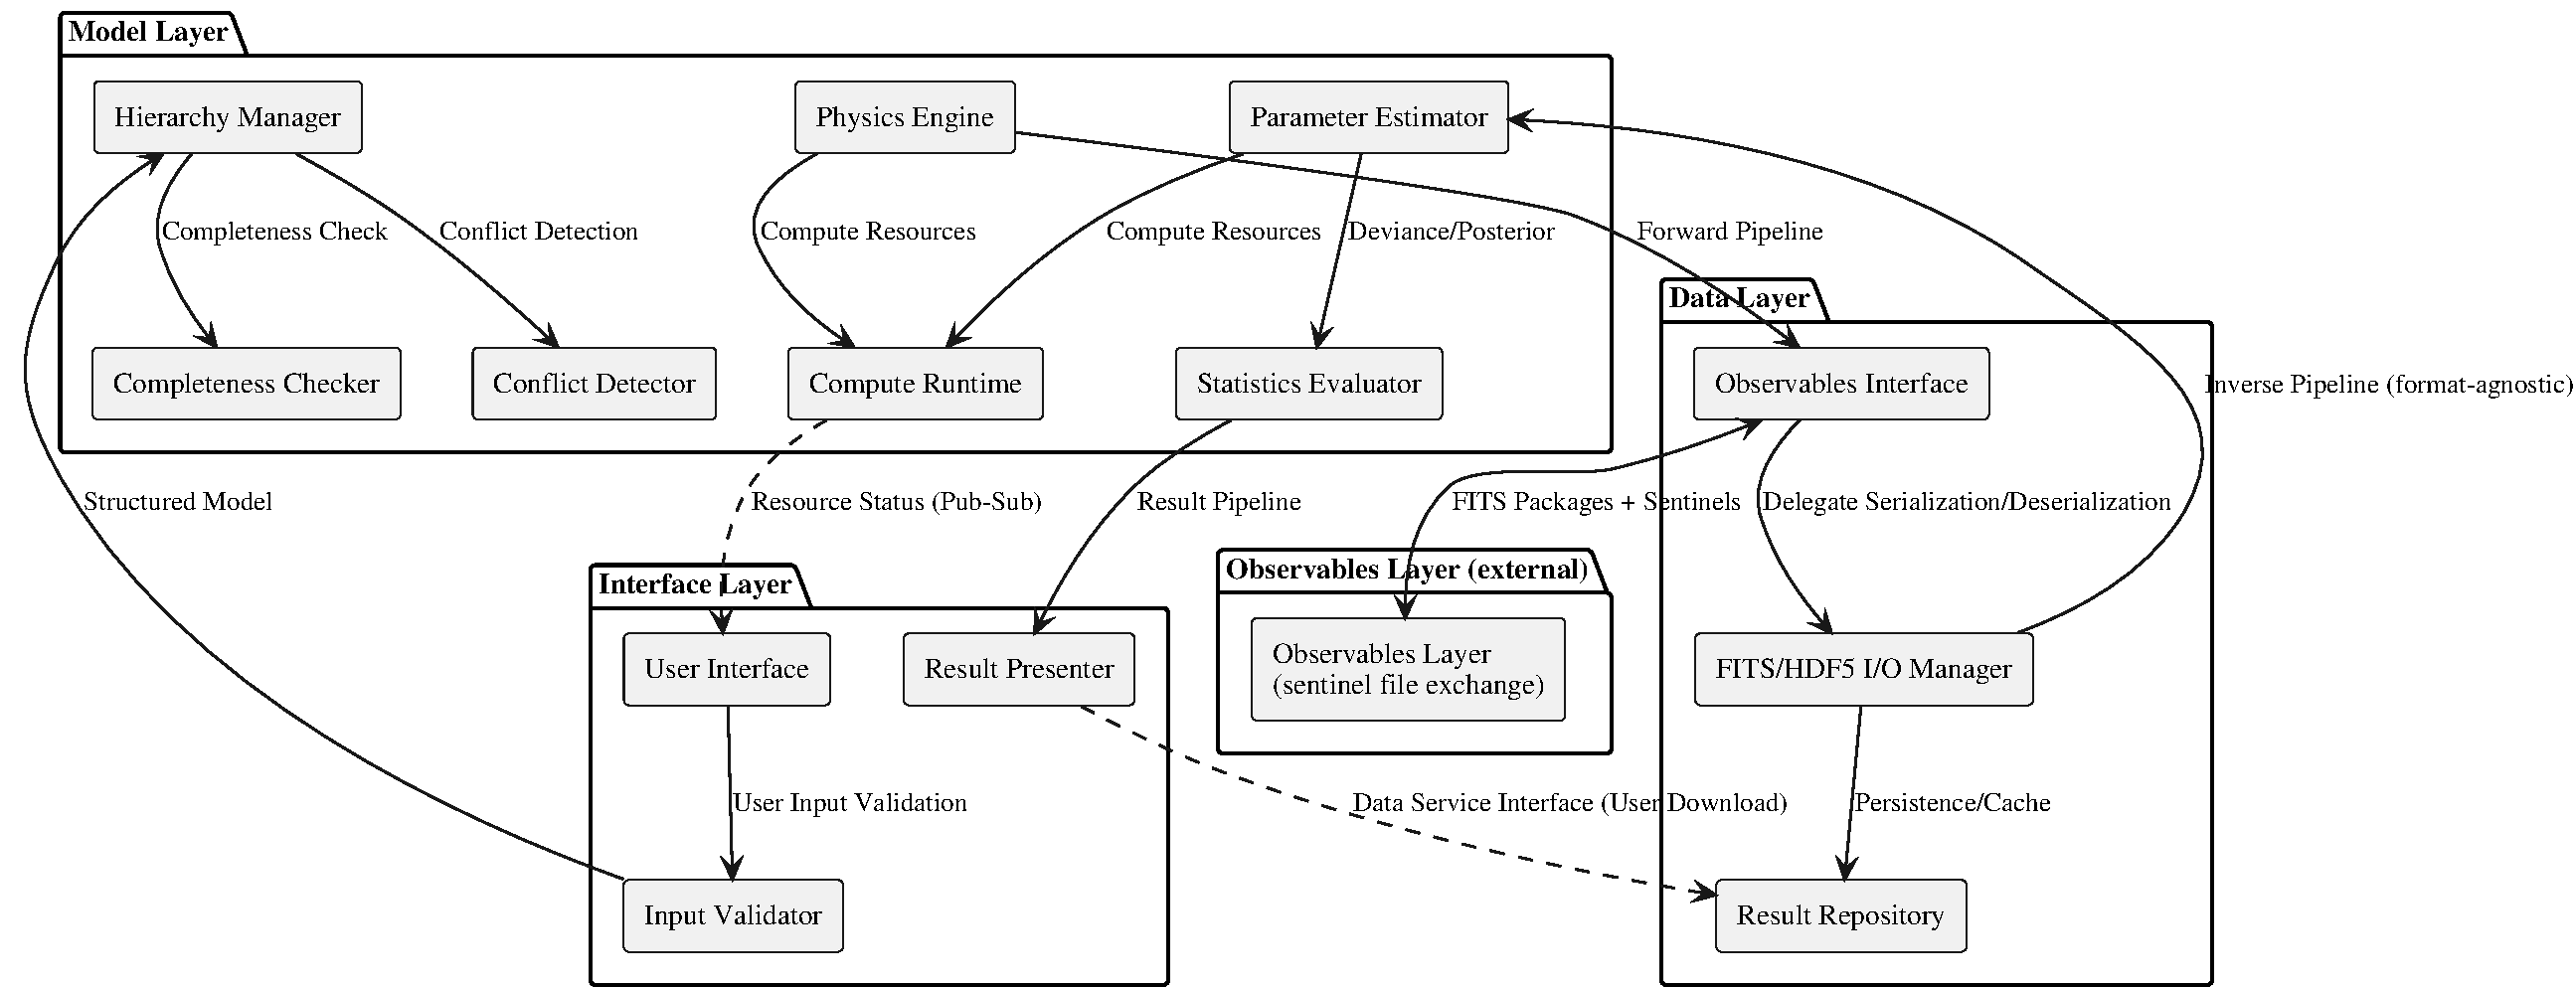
\includegraphics[width=0.98\textwidth]{components.pdf}
  \caption{目标层组件图（含与观测量层的边界）}
  \label{fig:components}
\end{figure}

\subsection{组件职责}

\begin{longtable}{p{4.2cm}p{1.8cm}p{8.8cm}}
\toprule
组件 & 所属段 & 职责摘要 \\
\midrule
\endhead
User Interface & 接口段 & 接收用户输入（CLI/API/自然语言），展示结果与资源状态；唯一外部边界 \\
Input Validator & 接口段 & 语法合法性、字段完整性与数据类型检查（物理语义交由模型段） \\
Hierarchy Manager & 模型段 & 五层级（基础$\rightarrow$主题$\rightarrow$方向$\rightarrow$任务$\rightarrow$目标）继承链管理、版本控制与命名空间隔离 \\
Conflict Detector & 模型段 & 参数物理不自洽、单位制合法性、非物理取值（超光速、负温度等）检测 \\
Completeness Checker & 模型段 & 计算依赖图断点检测，确保参数到可观测体的转换链完整 \\
Physics Engine & 模型段 & 综合源/背景/透过率模型执行数值仿真，生成 \texttt{TargetHistogram} 内存对象 \\
Parameter Estimator & 模型段 & 结合先验执行 MCMC/嵌套采样/最大似然反演，产出后验参数 \\
Statistics Evaluator & 模型段 & 偏离度（$\chi^2$、残差）、置信区间、模型选择准则与一致性评估 \\
Compute Runtime & 模型段 & 并行调度、异构计算、缓存管理、资源监视与准入评估 \\
Result Presenter & 接口段 & 生成用户级报告（JSON/YAML/Markdown/图表）；不编辑 FITS \\
Observables Interface & 数据段 & 层间交换目录管理、哨兵文件通知、正演/反演文件包组织 \\
FITS/HDF5 I/O Manager & 数据段 & FITS 序列化/反序列化（WCS 与元数据）；向上交付格式无关内存对象 \\
Result Repository & 数据段 & 持久化、缓存、版本快照与生命周期管理 \\
\bottomrule
\end{longtable}

\subsection{核心数据结构}

\begin{figure}[htbp]
  \centering
  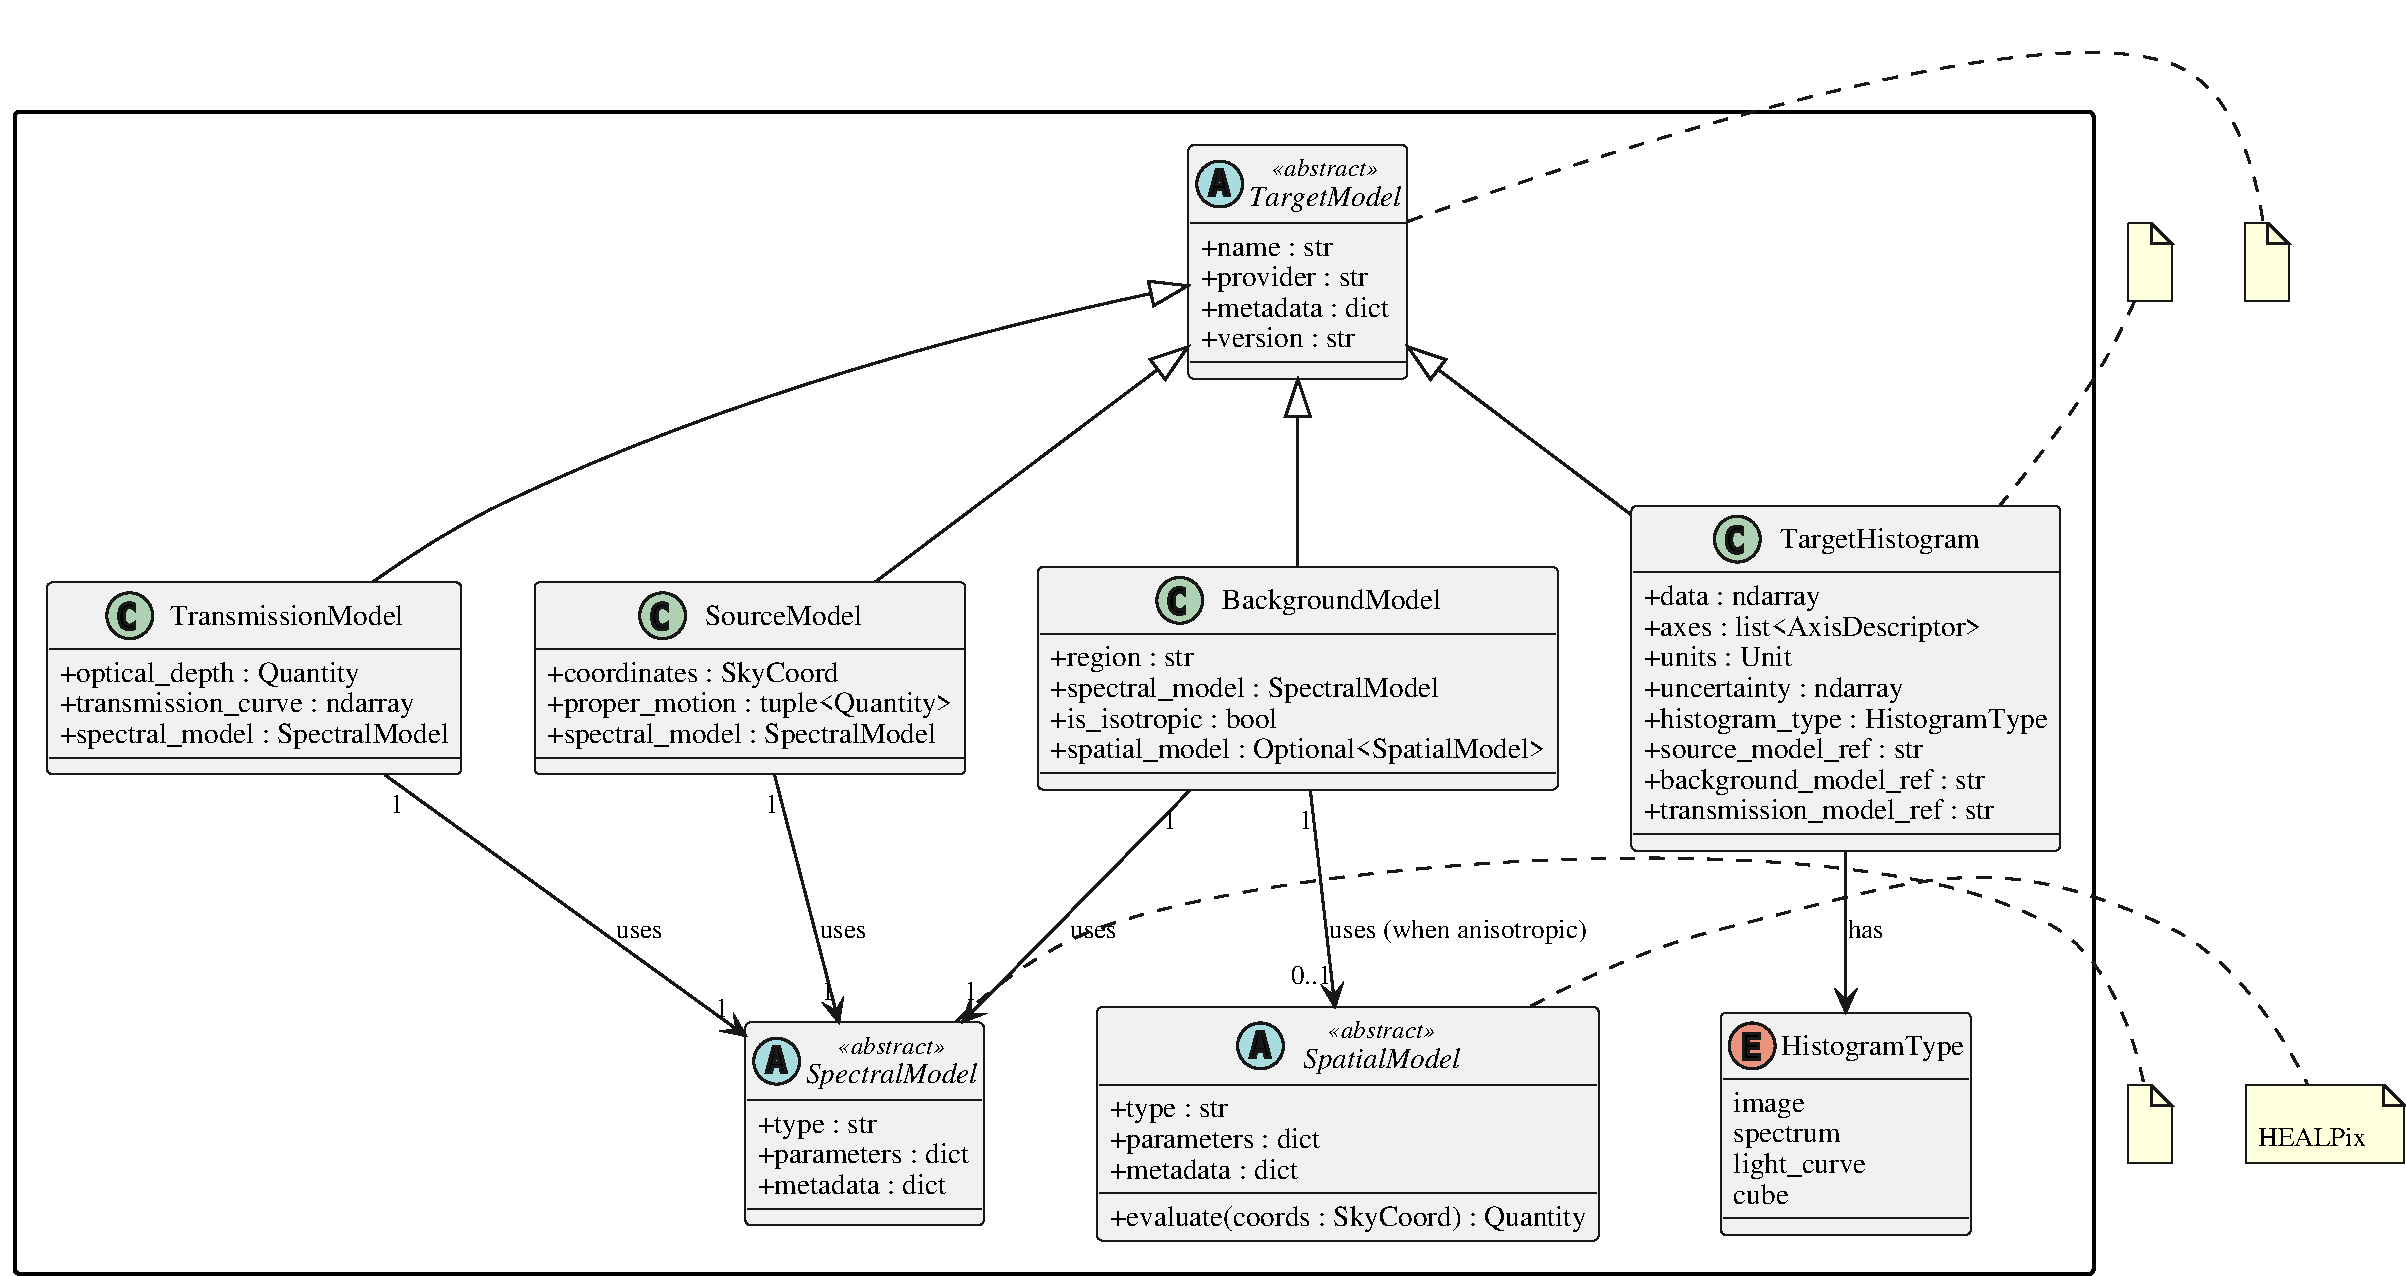
\includegraphics[width=\textwidth]{classes.pdf}
  \caption{目标层核心类图}
  \label{fig:classes}
\end{figure}

\begin{itemize}
  \item \texttt{TargetModel}：抽象基类，字段 \texttt{name} / \texttt{provider} / \texttt{version} /
        \texttt{metadata} / \texttt{hierarchy}；模型实例视为逻辑不可变，变更须递增版本。
  \item \texttt{SourceModel}：\texttt{coordinates}（SkyCoord 兼容）、\texttt{proper\_motion}、
        \texttt{spectral\_model}；\texttt{epoch}/\texttt{frame}（默认 J2000/ICRS）与可选星表块
        \texttt{catalogue}（ID/视差/测光，ADR 0009）。
  \item \texttt{DynamicalModel}（ADR 0008）：定位太阳系天体（小行星等）——\texttt{epoch}、
        \texttt{elements}（\texttt{a}/\texttt{e}/\texttt{i}/\texttt{raan}/\texttt{argp} 与 \texttt{M} 或 \texttt{Tp}）、
        \texttt{H}、可选 \texttt{category} 与位置快照序列；位置计算属物理引擎实现阶段。
  \item \texttt{BackgroundModel}：\texttt{region}、\texttt{spectral\_model}、\texttt{is\_isotropic}（默认 true）、
        \texttt{spatial\_model}（各向异性时必填，见 ADR 0006）。
  \item \texttt{TransmissionModel}：\texttt{optical\_depth}、\texttt{transmission\_curve}（可选，优先于参数化模型）、
        \texttt{spectral\_model}。
  \item \texttt{TargetHistogram}：统一亮度分布容器——\texttt{data}、\texttt{axes}、\texttt{units}、
        \texttt{uncertainty}、\texttt{histogram\_type}（image / spectrum / light\_curve / cube）与三个
        模型引用字段（源/背景/透过率），支持正演溯源与反演回写。
  \item \texttt{SpectralModel} / \texttt{SpatialModel}：对称的抽象描述符（\texttt{type} / \texttt{parameters} /
        \texttt{metadata}）；\texttt{SpatialModel.evaluate(coords)} 返回归一化或绝对亮度。
  \item 枚举：\texttt{HistogramType}、\texttt{AxisType}（spatial / spectral / temporal / other）。
  \item 关键不变量（节选）：\texttt{axes} 长度等于 \texttt{data.ndim}；\texttt{uncertainty} 与 \texttt{data}
        形状一致；\texttt{is\_isotropic=False} 时 \texttt{spatial\_model} 必填。
\end{itemize}

\subsection{内部接口（A--H）}
\label{sec:icd-internal}

段间接口遵循\emph{内存对象契约}：一律通过类型化、与文件格式无关的抽象数据交互；大数组经共享内存视图零拷贝传递。

\begin{longtable}{p{2.6cm}p{3.2cm}p{3.0cm}p{5.8cm}}
\toprule
接口 & 方向 & 实现途径 & 要点 \\
\midrule
\endhead
A 输入管道 & 接口段 $\rightarrow$ 模型段 & 函数调用（结构化内存对象） & 参数化模型、单位制声明、任务上下文与模式标识 \\
B 正演管道 & 模型段 $\rightarrow$ 数据段 & 共享内存视图 & \texttt{TargetHistogram} 大数组句柄，零拷贝写入 \\
C 反演管道 & 数据段 $\rightarrow$ 模型段 & 共享内存视图 & 解析后的科学数据产品、噪声与质量标记 \\
D 结果管道 & 模型段 $\rightarrow$ 接口段 & 函数调用 / 回调 & 拟合参数、统计量、诊断数据（禁止外部文件传输） \\
E 计算支撑 & 模型段 $\leftrightarrow$ Compute Runtime & 消息队列 + 共享内存句柄 & 任务描述、资源调度状态、缓存命中 \\
F 持久化支撑 & 数据段 $\leftrightarrow$ 结果仓库 & 进程内函数调用 & 存储/检索、缓存与生命周期（段内耦合） \\
G 数据服务 & 接口段 $\rightarrow$ 数据段（受控横向） & 请求-响应端口（Unix Domain Socket） & 用户级数据下载；禁止绕行模型段做科学计算交换 \\
H 资源状态 & 模型段 $\rightarrow$ 接口段 & 发布-订阅事件流 & 资源状态与准入评估推送（含降级建议） \\
\bottomrule
\end{longtable}

段间诊断导出（JSON/HDF5 文件）为受控补充途径，仅用于开发、测试与故障诊断，生产环境默认禁用。

\subsection{关键流程}

\begin{figure}[H]
  \centering
  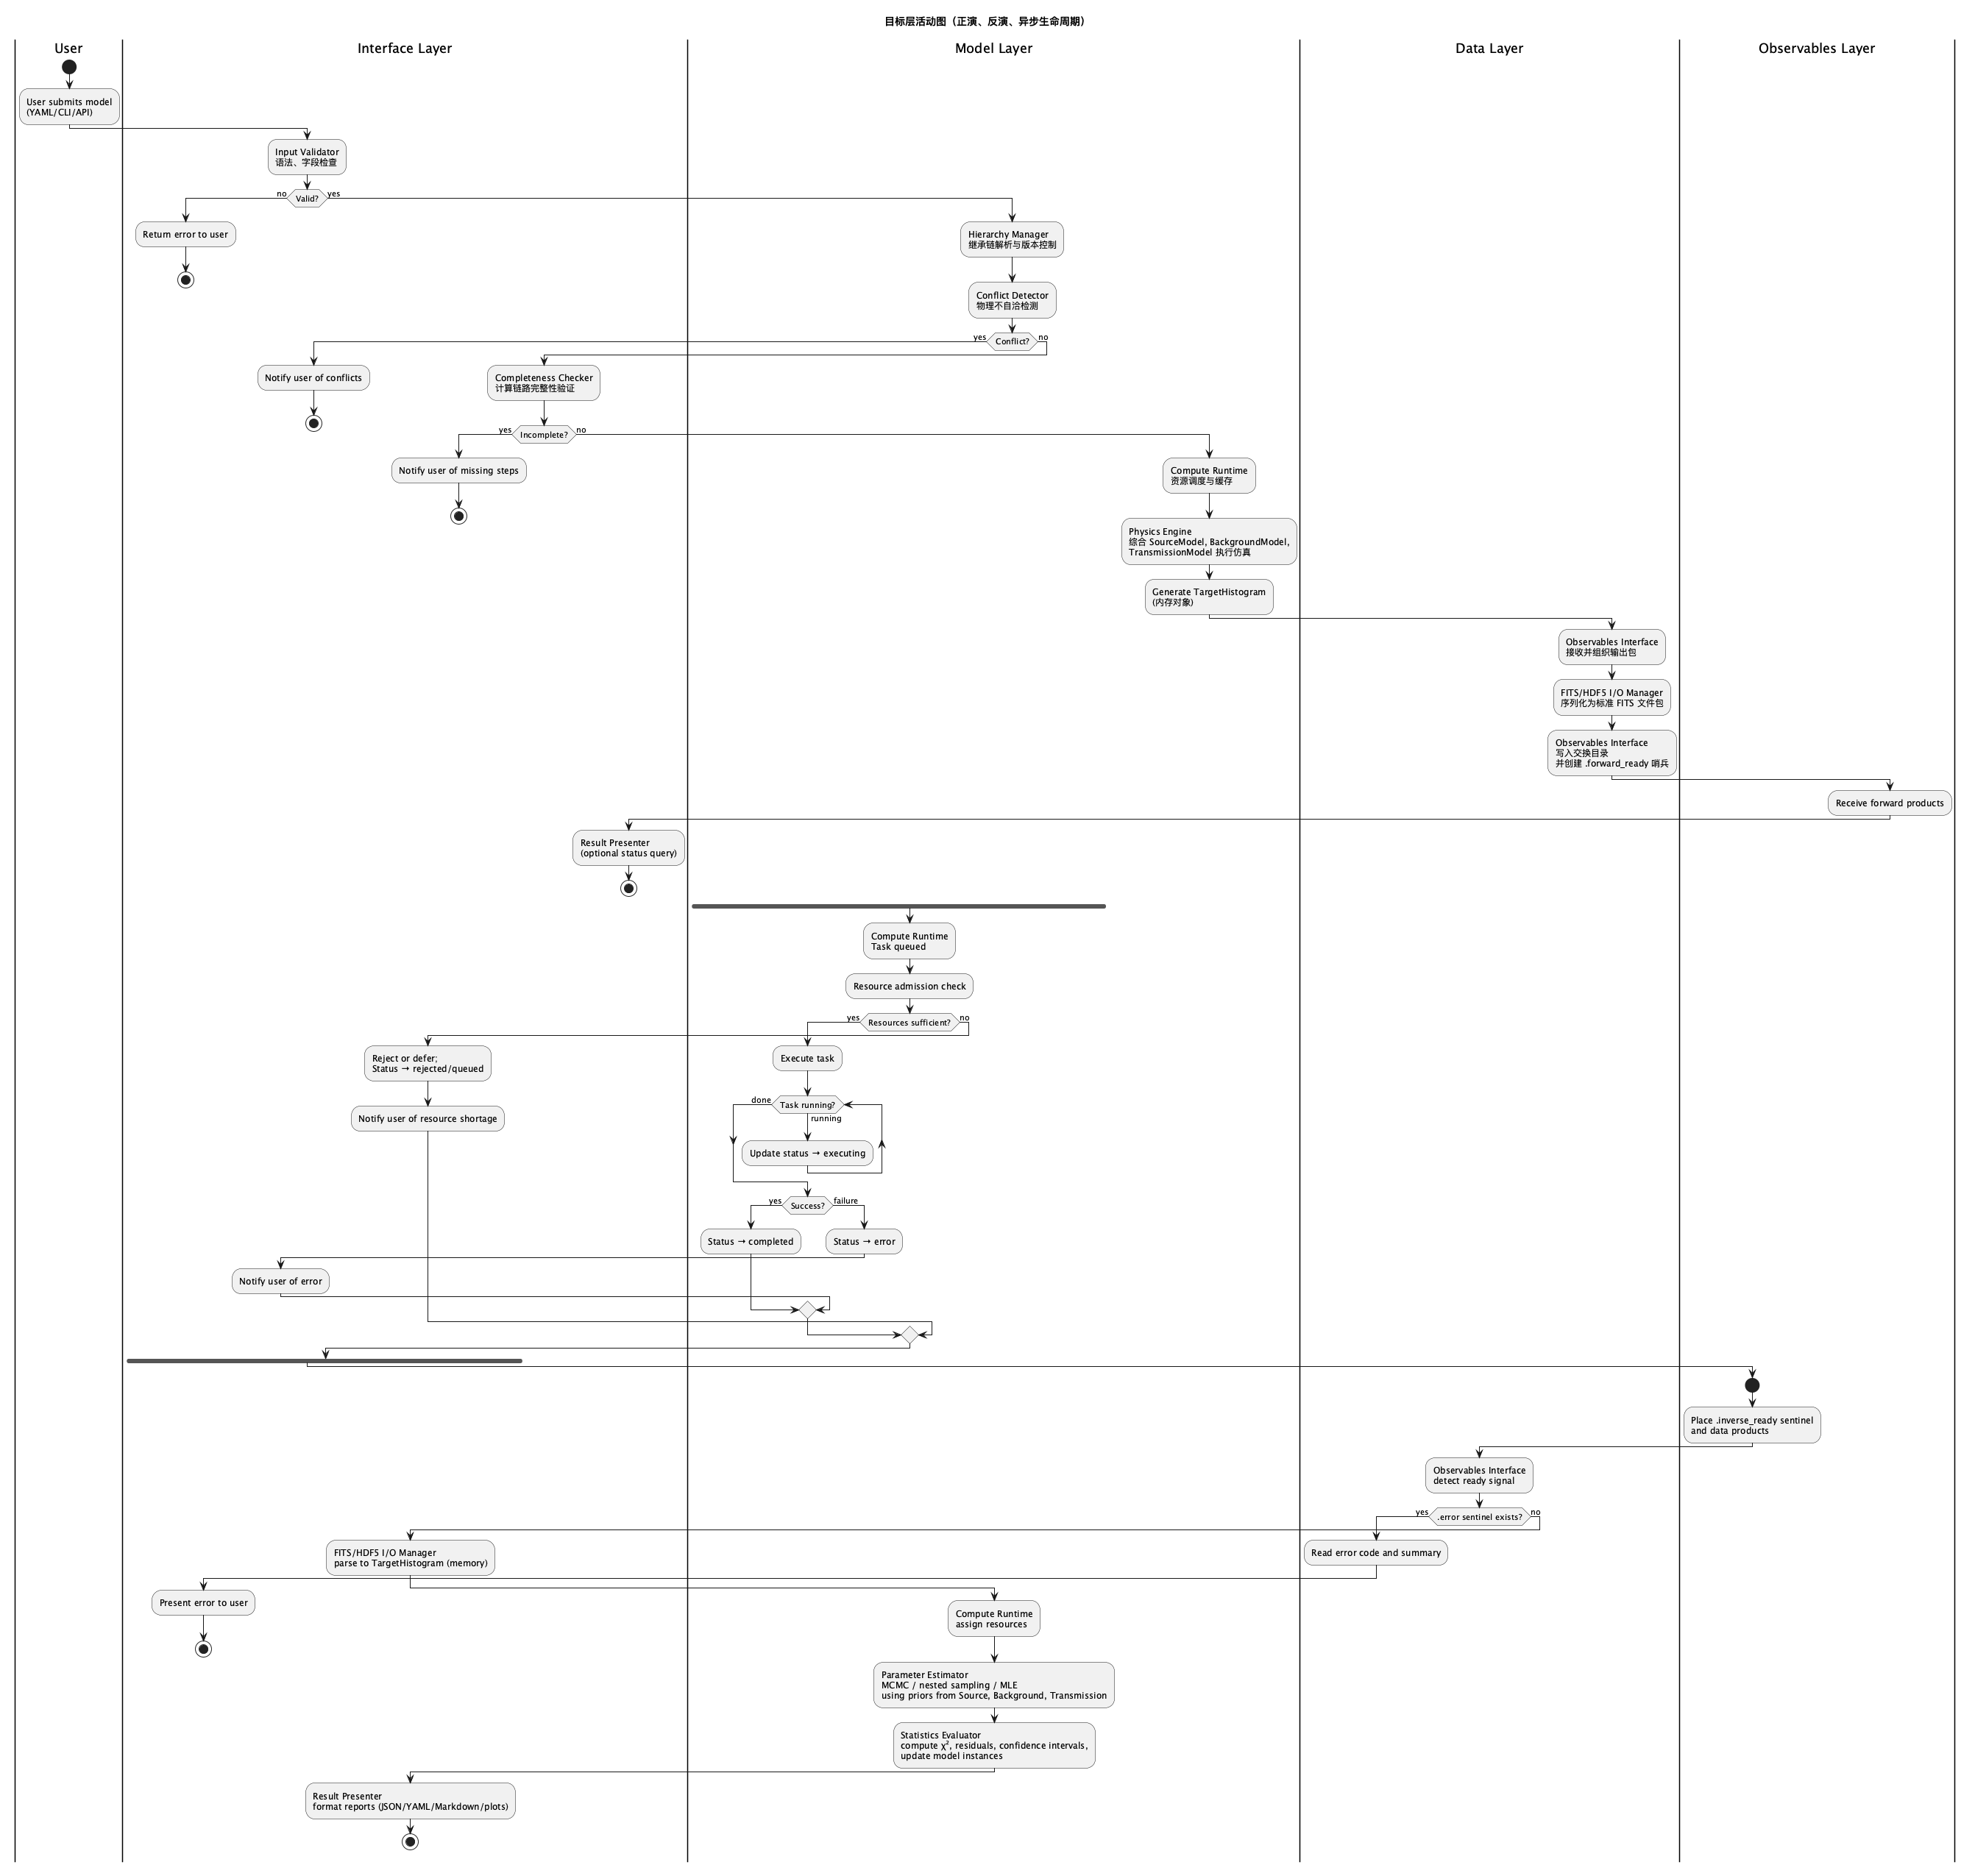
\includegraphics[width=\textwidth,height=0.82\textheight,keepaspectratio]{activities.png}
  \caption{目标层活动图（正演、反演与异步任务生命周期）}
  \label{fig:activities}
\end{figure}

\begin{itemize}
  \item \textbf{正演}：User Interface $\rightarrow$ Input Validator $\rightarrow$ Hierarchy Manager
        （冲突/完整性检测）$\rightarrow$ Compute Runtime 调度 $\rightarrow$ Physics Engine 仿真 $\rightarrow$
        \texttt{TargetHistogram} $\rightarrow$ Observables Interface $\rightarrow$ FITS I/O 序列化 $\rightarrow$
        交换目录 + \texttt{.forward\_ready} 哨兵。
  \item \textbf{反演}：\texttt{.inverse\_ready} 触发 $\rightarrow$ Observables Interface 检测 $\rightarrow$
        FITS I/O 解析为内存对象 $\rightarrow$ Parameter Estimator（结合先验）$\rightarrow$ Statistics Evaluator
        $\rightarrow$ Result Presenter 呈现报告。
  \item \textbf{异步生命周期与容错}：任务排队 $\rightarrow$ 资源准入（不足时拒绝/降级并通知）$\rightarrow$
        执行 $\rightarrow$ 完成/异常；观测层交换失败时读取 \texttt{.error} 错误码向上传播。
\end{itemize}
